\documentclass[11pt,a4paper]{article}
\usepackage[margin=22mm]{geometry}
\usepackage{amsmath,amssymb,graphicx,booktabs,longtable,array}
\usepackage[hidelinks]{hyperref}
\usepackage{microtype}
\graphicspath{{figs/}}
\setlength{\parskip}{2pt}
\newcommand{\sig}[1]{\sigma_{#1}}
\newcommand{\fittag}{C1\_with\_compass}
\newcommand{\chindf}{1.4018}
\newcommand{\chitot}{2140.5}
\newcommand{\ndf}{1527}
\newcommand{\npar}{28}
\newcommand{\nfit}{1555}
\newcommand{\rduHT}{-0.296}
\newcommand{\rduET}{0.935}
\newcommand{\rnoverp}{1.049}
\newcommand{\rsigLoversigT}{0.080}


\title{An amplitude-level model of $\pi^0$ and $\eta$ electroproduction\\
       fitted to CLAS, Hall A and COMPASS}
\author{V.\ Kubarovsky}
\date{6 September 2026 \quad--\quad fit \texttt{\fittag}}

\begin{document}
\maketitle

\begin{abstract}
\noindent
A model of exclusive $\pi^0$ and $\eta$ electroproduction is built directly at
the level of the helicity amplitudes, without reference to generalised parton
distributions, and fitted to \nfit{} measured points from CLAS6, CLAS12,
Hall A and COMPASS.  The purpose is not to test a particular GPD
parametrisation but to establish what the data themselves demand of the
amplitudes, so that any model can be measured against it.  The fit has \npar{}
free parameters and gives $\chi^2/\mathrm{ndf} = \chindf$ (\chitot/\ndf).
Four conclusions survive a full leave-one-out analysis: the flavour ratio
$n/p$ is separated by four neutron points and by nothing else; one
polarised-target
experiment alone fixes the relative phase of two transverse amplitudes;
$\sig{LT}$ is the model's systematic failure, seen independently in three data
sets; and a single power $Q^{n_Q}$ cannot span $Q^2$ from $1.2$ to
$8.3\ \mathrm{GeV}^2$.
\end{abstract}

\section{The model}

\subsection{Amplitudes}

The observables are built from six channel helicity amplitudes.  In the
notation of the $\pi^0$ amplitude note,
\[
\begin{array}{llll}
T_{00}^{(+)} & \text{longitudinal, recoil non-flip} &\quad
T_{00}^{(-)} & \text{longitudinal, recoil flip}\\
T_{01}^{(+)} & \text{natural transverse, non-flip} &\quad
T_{01}^{(-)} & \text{natural transverse, flip}\\
U_{01}^{(+)} & \text{unnatural transverse, non-flip} &\quad
U_{01}^{(-)} & \text{unnatural transverse, flip}
\end{array}
\]
At the level used here $T_{01}^{(-)} = U_{01}^{(-)} = D/2$, real and equal,
which is the forward-kinematics relation; the remaining four carry the fitted
moduli and phases.

The amplitudes are constructed from flavour generalised form factors.  Each
block $X \in \{H_T^u, H_T^d, \bar E_T^u, \bar E_T^d, L\}$ has the form
\begin{equation}
X(t, x_B, Q^2) \;=\; N \,
\exp\!\big[(b + b' \ln x_B)\, t\big]\;
\big(Q^2\big)^{n_Q/2},
\label{eq:gff}
\end{equation}
so that $b$ is the $t$-slope extrapolated to $x_B = 1$ and $-b'$ plays the role
of the Regge $\alpha'$.  This is the same convention as the Goloskokov--Kroll
fits.  Note that an older parameter convention used
$L = \ln x_B - \ln 0.15$; files in that convention must be converted, never
copied raw.

The flavour combinations entering each channel are
\begin{equation}
\pi^0 p:\ \frac{2X_u + X_d}{3\sqrt2}, \qquad
\eta\, p:\ \frac{2X_u - X_d}{3\sqrt6\,k}, \qquad
\pi^0 n:\ \frac{X_u + 2X_d}{3\sqrt2},
\end{equation}
with $k = 0.863$ in the transverse twist-3 sector (chiral condensate factors)
and $k = 0.695$ in the longitudinal twist-2 sector (decay constants only).
The near cancellation $2X_u - X_d$ in the $\eta$ channel is what makes that
channel sensitive to the flavour separation, and it is the reason $\eta$ data
carry weight far beyond their number.

Writing $\xi = \frac{x_B}{2-x_B}\left(1 + M_p^2/Q^2\right)$,
$t' = t - t_{\min}$ and $A = A(Q^2,x_B)$ for the phase-space factor,
\begin{equation}
D = \sqrt{2A\,(1-\xi^2)}\;\langle H_T\rangle, \qquad
U_{01}^{(+)} = \sqrt{A\,\kappa}\;\langle \bar E_T\rangle, \qquad
|T_{00}^{(-)}| = \sqrt{A\,\kappa}\;\langle L\rangle,
\end{equation}
with $\kappa = -t'/(8M_p^2)$ and $\langle\cdot\rangle$ the flavour combination
above.  Four further parameters unlock what would otherwise be exact
relations: $\rho_{CE}$ and $\phi_{CE}$ give $T_{01}^{(+)}$ a modulus and phase
relative to $U_{01}^{(+)}$ (breaking $C = E$), $\phi_w$ is the phase of
$U_{01}^{(+)}$, and $\rho_{nf}, \phi_{nf}$ give the longitudinal non-flip
amplitude $T_{00}^{(+)}$, which vanishes at leading order.  The phase of
$T_{00}^{(-)}$ is $\delta_0 + \delta_1 t$, common to both flavours.

Finally, each $d$-flavour convolution carries a phase relative to $u$.  The
overall phase of a channel is unobservable, so $u$ is kept real and only $d$
carries $\varphi_{d/u}$, separately for $H_T$, $\bar E_T$ and $L$.  These are
physical: the real and imaginary parts of a convolution have different
$t$-slopes, so $u$ and $d$ cannot share a phase, and the $\eta$ cancellation
therefore ceases to be exact.

\subsection{From amplitudes to structure functions}

The nine structure functions follow from the Fourier dictionary, verified in
the note against the QED photon density matrix:
\begin{align}
\sig{L} &= \textstyle\sum |T_{00}|^2, &
\sig{T} &= \textstyle\sum |T_{01}|^2 + \sum |U_{01}|^2, &
\sig{TT} &= \textstyle\sum |T_{01}|^2 - \sum |U_{01}|^2,\notag\\
\sig{LT} + i\,\sig{LT'} &= -\sqrt2 \textstyle\sum T_{00}^{*} T_{01}, &
\sig{LT'}^{LL} + i\,\sig{LT}^{UL} &= -\sqrt2 \textstyle\sum T_{00}^{*} U_{01}, &
\sig{T'} + i\,\sig{TT}^{UL} &= 2 \textstyle\sum T_{01}^{*} U_{01}.
\label{eq:gram}
\end{align}
Only the moduli of $T_{01}$ and $U_{01}$ enter $\sig{T}$ and $\sig{TT}$; their
\emph{relative phase} appears only in $\sig{T'}$.  This observation matters
later: it is why one polarised-target experiment is the sole constraint on that
phase.

The measured cross section is the standard decomposition
\begin{equation}
\frac{d^2\sigma}{dt\,d\phi} = \frac{1}{2\pi}\Big[
\sig{T} + \epsilon\,\sig{L}
+ \epsilon\cos 2\phi\; \sig{TT}
+ \sqrt{2\epsilon(1+\epsilon)}\cos\phi\; \sig{LT}
+ h\sqrt{2\epsilon(1-\epsilon)}\sin\phi\; \sig{LT'}\Big],
\label{eq:phidecomp}
\end{equation}
identical to eq.~(B4) of the CLAS6 paper and eq.~(2) of COMPASS, with $\phi$ in
the Trento convention and $h$ the beam helicity.

\section{The data}

Thirteen data sets are loaded from a single workbook,
\texttt{pi0\_eta\_database.xlsx}.  Nothing enters the fit from any other
source: a second source is how an old, mis-weighted version of one set once
survived unnoticed.  Table~\ref{tab:sets} lists everything, fitted or not.

\begin{table}[htb]
\centering\small
\caption{The database and the fit.  A set marked $--$ is not fitted; its
$\chi^2$ is then a blind prediction.  CLAS12 cross sections are preliminary;
the published De Masi $\alpha$ are the same measurement as the $\phi$
distributions and would be double counting.}
\label{tab:sets}
\begin{tabular}{llccrr}
\toprule
set & key & fitted & points & $\chi^2$ & per point \\
\midrule
CLAS6 $\pi^0$ p & \texttt{clas6\_pi0} & yes & 288 & 484.2 & 1.68 \\
CLAS6 $\eta$ p & \texttt{clas6\_eta} & yes & 207 & 216.3 & 1.04 \\
Hall A 2017, $\pi^0$ n & \texttt{halla\_n} & yes & 12 & 20.7 & 1.72 \\
Hall A 2016, $\pi^0$ p & \texttt{halla\_y16} & yes & 21 & 94.0 & 4.47 \\
Hall A 2011, $\pi^0$ p & \texttt{halla\_y11} & yes & 112 & 146.3 & 1.31 \\
Hall A 2021, $\pi^0$ p & \texttt{halla\_y21} & yes & 144 & 338.2 & 2.35 \\
CLAS12 cross sections & \texttt{clas12\_xs} & -- & 438 & 3830.9 & 8.75 \\
COMPASS 2025 & \texttt{compass} & yes & 26 & 64.9 & 2.49 \\
De Masi, published $\alpha$ & \texttt{bsa\_demasi} & -- & 56 & 81.7 & 1.46 \\
Zhao, $\eta$ BSA & \texttt{bsa\_zhao} & yes & 12 & 13.6 & 1.13 \\
CLAS12 $\sigma_{LT'}/\sigma_0$ & \texttt{bsa\_clas12} & yes & 30 & 46.1 & 1.54 \\
De Masi, $A_{LU}(\phi)$ & \texttt{bsa\_demasi\_phi} & yes & 663 & 620.7 & 0.94 \\
eg1-dvcs, pol.\ target & \texttt{eg1} & yes & 40 & 73.9 & 1.85 \\
\bottomrule
\end{tabular}

\end{table}

\subsection{Provenance of the uncertainties}

Every weight in the fit now comes from a publication.  Three defects were
repaired on 5 September 2026 and are recorded here because they changed the
answer, not merely the bookkeeping.

\paragraph{De Masi carried no systematic at all.}  The CLAS physics database
export gives statistical errors only, so 703 $\phi$ points were the most
heavily weighted set in the sample.  Ref.~PRC~\textbf{77} 042201(R), p.~3,
quotes $0.016$ from event selection and from the choice of fit function; it is
now applied to all 703 points and to the 62 published moments.

\paragraph{The Hall A neutron systematics exist only as a picture.}
PRL~\textbf{118} 222002 gives no table; the point-to-point uncertainties appear
only as the shaded bands of its figure~5.  They were read from the vector PDF,
with the vertical calibration taken not from the axis but from the published
error bars themselves --- half a bar in figure units against the quoted
statistical error.  The calibration closes to $0.0\,\%$ in the $\sig{T}$ panel
and $1.8\,\%$ in $\sig{LT}$ and $\sig{TT}$.  The bands are asymmetric, in
places by a factor three; they are symmetrised as (up + down)/2, and the
$3.1\,\%$ normalisation they contain is removed in quadrature because it is
fitted separately.

\paragraph{An invented 10\,\% was removed.}  Hall A 2016 and the neutron had
been carrying a flat 10\,\% of the author's own making.  It was wrong in both
directions at once: it concealed a real discrepancy in the 2016 proton set
(3.93 $\to$ 5.78 per point once removed) and inflated a false one in the
neutron, whose true bands are larger than 10\,\%.  An invented uncertainty is
worse than a missing one, because it looks like knowledge.

\subsection{Normalisation uncertainties}

Three sets carry an overall normalisation that multiplies every point together:
$3.5\,\%$ for De Masi (beam polarisation), $3.12\,\%$ for Hall A 2016
(ref.~PRL~\textbf{117} 262001, table III) and $3.1\,\%$ for the neutron.  Adding
these in quadrature to the per-point errors would discard the correlation and
smear each set instead of letting it move as a whole.  They are therefore
fitted as one free scale per set,
\begin{equation}
r = \frac{\text{data} - \lambda\,\text{model}}{\sigma},
\qquad\text{with a penalty}\quad \left(\frac{\lambda-1}{\sigma_{\rm norm}}\right)^2
\ \text{counted in }\chi^2,
\end{equation}
and the number of degrees of freedom reduced by the number of $\lambda$;
otherwise a nuisance would be a free way to improve $\chi^2/\mathrm{ndf}$.
Table~\ref{tab:norms} gives the results.  Hall A 2016 is the one to notice: its
normalisation is dragged nearly two standard deviations and the set still does
not fit.

\begin{table}[htb]
\centering\small
\caption{Fitted normalisations.}
\label{tab:norms}
\begin{tabular}{lccc}
\toprule
set & prior & $\lambda$ & pull \\
\midrule
\texttt{bsa\_demasi\_phi} & $3.50\,\%$ & $1.0587 \pm 0.0326$ & $+1.68\,\sigma$ \\
\texttt{halla\_n} & $3.10\,\%$ & $0.9776 \pm 0.0304$ & $-0.72\,\sigma$ \\
\texttt{halla\_y16} & $3.12\,\%$ & $1.0562 \pm 0.0253$ & $+1.80\,\sigma$ \\
\bottomrule
\end{tabular}

\end{table}

\section{The fit}

\subsection{Constraints}

Two constraints are imposed for stated physical reasons rather than to improve
$\chi^2$.

\paragraph{$n_{Q,d} = n_{Q,u}$ in both transverse sectors.}  A generalised form
factor is (GPD) $\times$ (hard subprocess).  The GPD carries no $Q^2$
dependence, and the subprocess is flavour-blind up to the quark charge.
Transversity does not mix with gluons, so its evolution is non-singlet and
flavour-blind as well.  Left free, the fitted $n_{Q,d} - n_{Q,u}$ came out
$-7.0$ and $+2.8$ in successive fits, with flavour ratios running by an order
of magnitude across $Q^2$.

\paragraph{$b_d = b_u$ for $H_T$.}  Left free, the fit drives $b_d$ to whatever
ceiling it is given --- 12, 18, 25 --- buying two units of $\chi^2$ while the
normalisation $N_d$ compensates by a factor sixteen.  It is a flat valley, not
a measurement.

In addition every $t$-slope is required non-negative over $x_B \in [0.05,1]$,
not only where there are data: without it $H_T^u$ came out with $b=-0.26$, so
that the form factor \emph{grew} with $|t|$ above $x_B = 0.785$.

\subsection{Parameters}

Tables~\ref{tab:blocks} and~\ref{tab:other} give all \npar{} fitted
parameters with errors from the Jacobian at the minimum.  A dagger marks a
parameter sitting on a bound, where the quoted error is one-sided and the value
is not a measurement.

\begin{table}[htb]
\centering\small
\caption{Block parameters, eq.~(\ref{eq:gff}).  $N$ in nb$^{1/2}$/GeV,
$b$ and $b'$ in GeV$^{-2}$, $n_Q$ dimensionless.}
\label{tab:blocks}
\begin{tabular}{lcccc}
\toprule
block & $N$ & $b$ & $b'$ & $n_Q$ \\
\midrule
$H_T^u$ & $20.633 \pm 0.626$ & $0.000 \pm 0.043$$^{\dagger}$ & $-1.086 \pm 0.061$ & $1.227 \pm 0.031$ \\
$H_T^d$ & $-6.480 \pm 5.490$ & $=b_u$ & $=b_u'$ & $=n_{Q,u}$ \\
$\bar E_T^u$ & $60.785 \pm 2.884$ & $0.678 \pm 0.049$ & $-0.312 \pm 0.036$ & $1.164 \pm 0.065$ \\
$\bar E_T^d$ & $229.131 \pm 21.224$ & $5.366 \pm 0.358$ & $=b_u'(\bar E_T)$ & $=n_{Q,u}(\bar E_T)$ \\
$L$ (T00) & $36.118 \pm 4.442$ & $0.000 \pm 0.043$$^{\dagger}$ & $-1.269 \pm 0.104$ & $0.390 \pm 0.144$ \\
\bottomrule
\end{tabular}

\end{table}

\begin{table}[htb]
\centering\small
\caption{Remaining parameters, with the interval each was allowed.}
\label{tab:other}
\begin{tabular}{lccc}
\toprule
parameter & value & lower & upper \\
\midrule
$R_L=N_d/N_u$ (T00) & $-0.652 \pm 0.177$ & -2.00 & 2.00 \\
$\delta_0$ & $1.727 \pm 0.082$ & -3.14 & 3.14 \\
$\delta_1$ & $0.695 \pm 0.088$ & -3.00 & 3.00 \\
$\rho_{CE}$ & $0.170 \pm 0.021$ & 0.00 & 1.50 \\
$\phi_{CE}$ (frozen) & $0.000 \pm 0.000$ & -3.14 & 3.14 \\
$\phi_w$ & $-0.586 \pm 0.125$ & -3.14 & 3.14 \\
$\rho_{nf}$ & $1.726 \pm 0.201$ & 0.00 & 3.00 \\
$\phi_{nf}$ & $2.107 \pm 0.148$ & -3.14 & 3.14 \\
$\varphi_{d/u}(H_T)$ & $-1.254 \pm 0.277$ & -3.14 & 3.14 \\
$\varphi_{d/u}(\bar E_T)$ & $0.179 \pm 0.451$ & -3.14 & 3.14 \\
$\varphi_{d/u}(T_{00})$ & $0.502 \pm 0.337$ & -3.14 & 3.14 \\
\bottomrule
\end{tabular}

\end{table}

Two features deserve comment.  $N_d$ of $H_T$ is consistent with zero: the
$d$-quark transversity normalisation is not determined by these data at all.
And the $d/u$ phase of $\bar E_T$ is likewise consistent with zero, while only
the $H_T$ phase differs from zero, by about $4.5\sigma$.

\subsection{Derived quantities}

At $Q^2 = 1.75\ \mathrm{GeV}^2$, $x_B = 0.36$, $-t = 0.27\ \mathrm{GeV}^2$:
\[
\frac{d}{u}\Big|_{H_T} = \rduHT, \qquad
\left|\frac{d}{u}\right|_{\bar E_T} = \rduET, \qquad
\frac{n}{p}\Big|_{\sig{TT}} = \rnoverp, \qquad
\frac{\sig{L}}{\sig{T}} = \rsigLoversigT .
\]
The $n/p$ ratio carries a caveat that is not a formality; see
section~\ref{sec:notmeasured}.

\section{What the leave-one-out analysis shows}

Each data set was removed in turn and the fit repeated, in two series: without
and with Hall A 2021.  A set's $\chi^2$ when it is \emph{not} fitted is a blind
prediction, and is the useful number: a set that is left out and still
described brings no unique information.

\begin{table}[htb]
\centering\small
\caption{Blind $\chi^2$ per point of the set that was removed, and the effect
on two derived quantities.  Series~8 has 9 sets and no Hall A 2021; series~D has 10, with it, and is fitted to the corrected $x_B$.}
\label{tab:loo}
\begin{tabular}{lccrr}
\toprule
removed & blind, series 8 & blind, series D & $d/u|_{H_T}$ & $n/p$\\
\midrule
--- (reference) & --- & --- & $-0.314$ & $1.070$\\
CLAS6 $\pi^0$ & 2.89 & 3.69 & $-0.328$ & 0.974\\
CLAS6 $\eta$ & \textbf{218.9} & \textbf{2.90} & $-0.463$ & 1.236\\
Hall A neutron & 10.06 & \textbf{13.48} & $+0.407$ & \textbf{2.195}\\
Hall A 2016 & 6.18 & 6.03 & $-0.340$ & 1.046\\
Hall A 2011 & 2.66 & 1.81 & $-0.348$ & 1.098\\
Hall A 2021 & --- & 11.05 & $-0.238$ & 1.037\\
De Masi $\phi$ & 1.02 & 1.02 & $-0.283$ & 1.080\\
Zhao & 2.25 & 1.73 & $-0.247$ & 1.093\\
CLAS12 BSA & 2.88 & 2.59 & $-0.335$ & 1.055\\
eg1-dvcs & \textbf{40.16} & \textbf{66.54} & $-0.403$ & 0.652\\
\bottomrule
\end{tabular}
\end{table}

\paragraph{Hall A 2021 has taken the flavour separation over from $\eta$.}
Without it, removing the $\eta$ data left the model predicting $\eta$ at 219
per point.  With it in the fit that collapses to 2.90.  Hall A 2021 reaches
$x_B = 0.60$, the highest in the database, and now covers the region that only
the $\eta$ cancellation used to probe.  $\eta$ still moves $d/u|_{H_T}$ from
$-0.314$ to $-0.463$ when dropped; it is no longer irreplaceable.

\paragraph{The reference fit is reproducible.}  Removing Hall A 2021 from
series~D reproduces the series~8 reference to four figures, from a different
starting point.  The minima are real and not wherever the optimiser happened to
land.

\section{What the data determine weakly, or not at all}
\label{sec:notmeasured}

This section is the point of the exercise, and is stated as plainly as the
numbers allow.

\paragraph{$n/p$ is soft against the model, not only against the data.}
The neutron channel is $\langle X\rangle \propto X_u + 2X_d$ against the
proton's $2X_u + X_d$, so the $d$ block enters the neutron with twice the weight
it has in the proton.  Since $\sig{TT} = \sum|T_{01}|^2 - \sum|U_{01}|^2$ and
$U_{01}$ is built from $\bar E_T$, the ratio $n/p$ in $\sig{TT}$ is essentially a
statement about $\bar E_T^d$ relative to $\bar E_T^u$.

The fitted $t$-slopes of those two blocks differ by a factor eight,
$b_d = 5.28 \pm 0.36$ against $b_u = 0.67 \pm 0.05$.  That invites the suspicion
that it is the flat valley which forced $b_d = b_u$ in the $H_T$ sector, where
the same tie costs two units of $\chi^2$.  It is not: tying them in
$\bar E_T$ costs $194.5$ units for one parameter, which excludes the tie
decisively.

But look at who pays.  The cost falls on the \emph{proton} sets --- CLAS6
$\pi^0$ $+73.8$, Hall A 2016 $+50.3$, eg1 $+34.7$, Hall A 2011 $+26.8$ --- while
the neutron, the set whose four points are supposed to be carrying this ratio,
fits \emph{better} under the tie, $1.72 \to 0.65$ per point, and CLAS6 $\eta$
improves as well.  Under that constrained variant $n/p$ is $0.52$ instead of
$1.05$: half the value, at a $\chi^2$ the neutron itself prefers.

So the steep $d$ slope is a requirement of the proton data, and the neutron
points do not pin $n/p$ --- they are comfortable with a value twice smaller.
The quoted $\rnoverp$ is what the unconstrained fit returns, and the $194$ units
say the data prefer it, but the number is soft against a change of model
assumption in a way that no error bar expresses.  Its history over one day of
minor and justified changes --- corrected systematics, a normalisation nuisance,
a repaired bound, a corrected $x_B$ --- runs $1.00$, $1.02$, $0.98$, $1.04$,
$1.06$, $1.05$, with $\chi^2/\mathrm{ndf}$ moving in the third decimal.  A fifth
neutron point would be worth more than a thousand proton points, and a
measurement that constrained $\bar E_T^d$ directly would be worth more still.

\paragraph{One experiment fixes a phase.}  $\sig{T'} = 2\,\mathrm{Re}\langle
T_{01}, U_{01}\rangle$ by eq.~(\ref{eq:gram}); the unpolarised data fix only the
moduli.  The $A_{LL}$ moments of eg1-dvcs are the only observable in the
database that sees this interference, and when eg1 is left out its own blind
$\chi^2$ is 41 per point, with $\phi_w$ swinging from $-0.70$ to $+2.90$ ---
essentially a sign flip of $\sig{T'}$.  Forty points from one experiment.

\paragraph{$\sig{LT}$ is a systematic failure of the model.}  It is the worst
described quantity in three independent sets: 20.4 per point in the blind
prediction of the CLAS12 cross sections, 4.7 in Hall A 2016, and the worst of
the four observables in Hall A 2021.  Since $\sig{LT}$ carries the entire
$\cos\phi$ modulation of eq.~(\ref{eq:phidecomp}), any event generator built on
this model will inherit the failure in the shape of its $\phi$ distribution.

\paragraph{A single power of $Q^2$ does not span the range.}  Hall A 2016 and
Hall A 2021 disagree with the model in opposite directions at the two ends: at
$Q^2 = 1.5$ the model undershoots $\sig{T}$ ($1616 \pm 145$ measured against
1135), at $Q^2 = 8.3$ it overshoots $\sig{U}$ by a factor 1.8.  Hall A 2016
does not fit at all --- 4.5 per point with its normalisation already dragged
$1.8\sigma$ --- and these are the only Rosenbluth-separated proton points that
exist.  Admitting Hall A 2021 to the fit brings it from 13.1 to 2.34 per point,
but the asymmetries pay: eg1 from 1.36 to 1.81, the CLAS12 beam-spin asymmetry
from 1.04 to 1.53.  The compromise is real and it is visible.

\section{Comparison with Goloskokov--Kroll}

Two independent comparisons put the GK prediction for $\sig{LT'}$ far below the
data.  The published GK curve for the $\eta$ beam-spin asymmetry
(Zhao~\textit{et al.}, PLB~\textbf{789} 426, figure~5) is near zero across all
four bins where the data are $0.1$ to $0.3$.  For $\pi^0$, a GK calculation over
the 60 De Masi bins gives $\alpha \approx 0.01$--$0.025$ against a published
median of $0.080$.  The present model gives a median $0.077$ on the same bins,
but that is a fit, not a prediction; the fair statement is that when the De Masi
$\phi$ distributions are removed from the fit entirely they are still predicted
at 1.02 per point, so the magnitude of $\sig{LT'}$ demanded by all the
\emph{other} data is about five times what GK produces.

Throughout, $\alpha$ is the amplitude of $A_{LU} = \alpha\sin\phi/(1 + \beta
\cos\phi + \gamma\cos 2\phi)$ with $A_{LU}$ already divided by the beam
polarisation, so
$\alpha = \sqrt{2\epsilon(1-\epsilon)}\,\sig{LT'}/(\sig{T}+\epsilon\sig{L})$ and
not the bare ratio.

\clearpage
\section{Figures}

Every figure shows the data of one set against the fit.  A title reading
\textsc{not in the fit} marks a blind prediction.  Data are drawn in red, the
model in blue.  Each panel carries its own kinematics and $\chi^2$; the model
curve includes the fitted normalisation of
table~\ref{tab:norms} where the set has one, so the curve is what the fit
actually compares against the points.

\begin{figure}[p]\centering

\includegraphics[width=\textwidth]{00_chi2_summary.png}
\caption{All thirteen sets at a glance: $\chi^2$ per point, fitted and blind.}
\end{figure}

\begin{figure}[p]\centering

\includegraphics[width=\textwidth]{02_clas6_pi0_in_U.png}
\caption{CLAS6 $\pi^0$, $\sig{U} = \sig{T} + \epsilon\sig{L}$, with
re-computed radiative corrections.}
\end{figure}

\begin{figure}[p]\centering

\includegraphics[width=\textwidth]{02_clas6_pi0_in_LT.png}
\caption{CLAS6 $\pi^0$, $\sig{LT}$.}
\end{figure}

\begin{figure}[p]\centering

\includegraphics[width=\textwidth]{02_clas6_pi0_in_TT.png}
\caption{CLAS6 $\pi^0$, $\sig{TT}$.}
\end{figure}

\begin{figure}[p]\centering

\includegraphics[width=\textwidth]{03_clas6_eta_in_U.png}
\caption{CLAS6 $\eta$, $\sig{U}$.  This channel probes $2X_u - X_d$.}
\end{figure}

\begin{figure}[p]\centering

\includegraphics[width=\textwidth]{03_clas6_eta_in_LT.png}
\caption{CLAS6 $\eta$, $\sig{LT}$.}
\end{figure}

\begin{figure}[p]\centering

\includegraphics[width=\textwidth]{03_clas6_eta_in_TT.png}
\caption{CLAS6 $\eta$, $\sig{TT}$.}
\end{figure}

\begin{figure}[p]\centering

\includegraphics[width=0.72\textwidth]{04_halla_n_in_T.png}\\

\includegraphics[width=0.72\textwidth]{04_halla_n_in_LT.png}
\caption{Hall A 2017, $\pi^0$ off the \emph{neutron}: $\sig{T}$ and
$\sig{LT}$.  Four points, uncertainties of 42 to 90\,\%, and the sole
constraint on $n/p$.}
\end{figure}

\begin{figure}[p]\centering

\includegraphics[width=0.72\textwidth]{04_halla_n_in_TT.png}\\

\includegraphics[width=0.72\textwidth]{05_halla_y16_in_T.png}
\caption{Neutron $\sig{TT}$ (top) and Hall A 2016 proton $\sig{T}$ (bottom).
The latter is the worst-described set in the fit at 4.5 per point, with its
normalisation already pulled $1.8\sigma$.}
\end{figure}

\begin{figure}[p]\centering

\includegraphics[width=0.72\textwidth]{05_halla_y16_in_LT.png}\\

\includegraphics[width=0.72\textwidth]{05_halla_y16_in_TT.png}
\caption{Hall A 2016, $\sig{LT}$ and $\sig{TT}$.}
\end{figure}

\begin{figure}[p]\centering

\includegraphics[width=\textwidth]{06_halla_y11_in_U.png}
\caption{Hall A 2011, $\sig{U}$.  This set is published in the
Drechsel--Tiator normalisation; $\sig{LT}$ and $\sig{LT'}$ are converted by
$\gamma = 2M x_B/\sqrt{Q^2}$ before comparison.}
\end{figure}

\begin{figure}[p]\centering

\includegraphics[width=0.72\textwidth]{06_halla_y11_in_LT.png}\\

\includegraphics[width=0.72\textwidth]{06_halla_y11_in_TT.png}
\caption{Hall A 2011, $\sig{LT}$ and $\sig{TT}$.}
\end{figure}

\begin{figure}[p]\centering

\includegraphics[width=\textwidth]{06_halla_y11_in_LTp.png}
\caption{Hall A 2011, $\sig{LT'}$.}
\end{figure}

\begin{figure}[p]\centering

\includegraphics[width=\textwidth]{07_halla_y21_in_U.png}
\caption{Hall A 2021, $\sig{U}$.  The only data above $Q^2 = 4.3$, reaching
$8.31\ \mathrm{GeV}^2$; left out of the fit the model overshoots these points
by a factor 1.8.}
\end{figure}

\begin{figure}[p]\centering

\includegraphics[width=0.72\textwidth]{07_halla_y21_in_LT.png}\\

\includegraphics[width=0.72\textwidth]{07_halla_y21_in_TT.png}
\caption{Hall A 2021, $\sig{LT}$ and $\sig{TT}$.}
\end{figure}

\begin{figure}[p]\centering

\includegraphics[width=\textwidth]{07_halla_y21_in_LTp.png}
\caption{Hall A 2021, $\sig{LT'}$.}
\end{figure}

\begin{figure}[p]\centering

\includegraphics[width=\textwidth]{08_clas12_xs_out_U.png}
\caption{CLAS12 cross sections, $\sig{U}$ --- \emph{not} in the fit, and
preliminary.  Predicted at 2.39 per point.}
\end{figure}

\begin{figure}[p]\centering

\includegraphics[width=\textwidth]{08_clas12_xs_out_LT.png}
\caption{CLAS12, $\sig{LT}$, blind: 20.4 per point.  This is the clearest
single picture of the model's failure in $\sig{LT}$.}
\end{figure}

\begin{figure}[p]\centering

\includegraphics[width=\textwidth]{08_clas12_xs_out_TT.png}
\caption{CLAS12, $\sig{TT}$, blind: 3.51 per point.}
\end{figure}

\begin{figure}[p]\centering
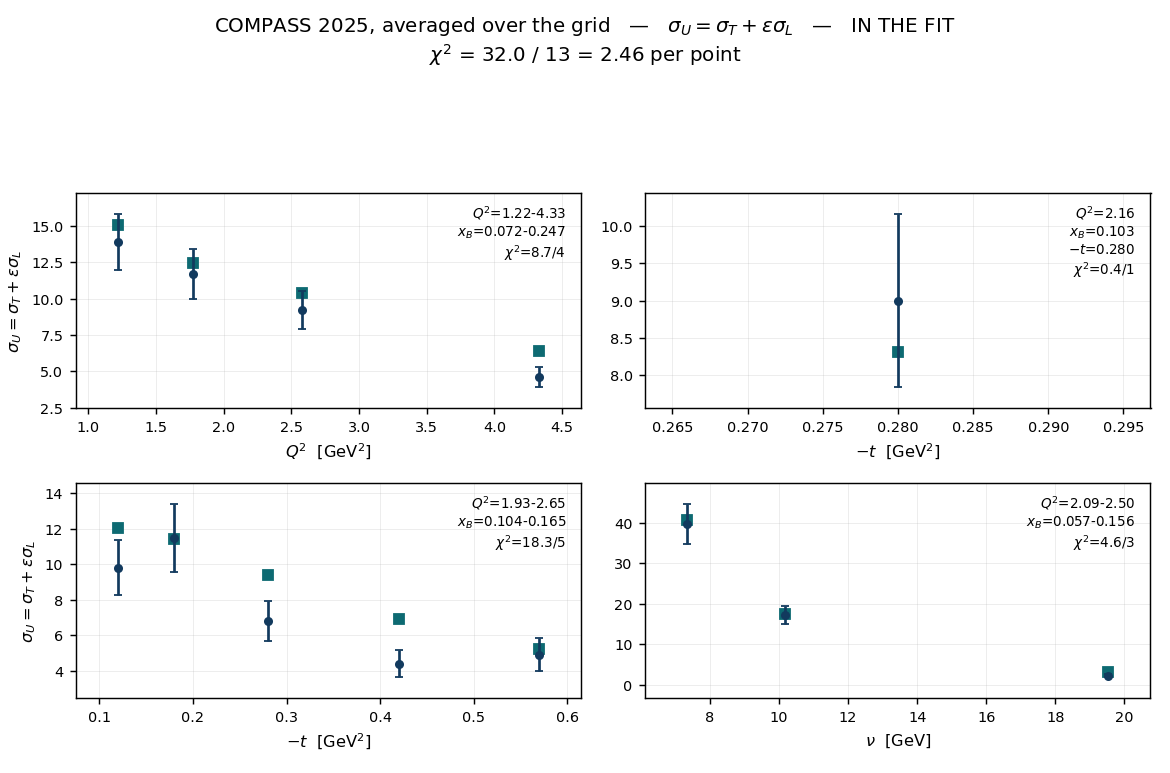
\includegraphics[width=0.72\textwidth]{09_compass_in_U.png}\\
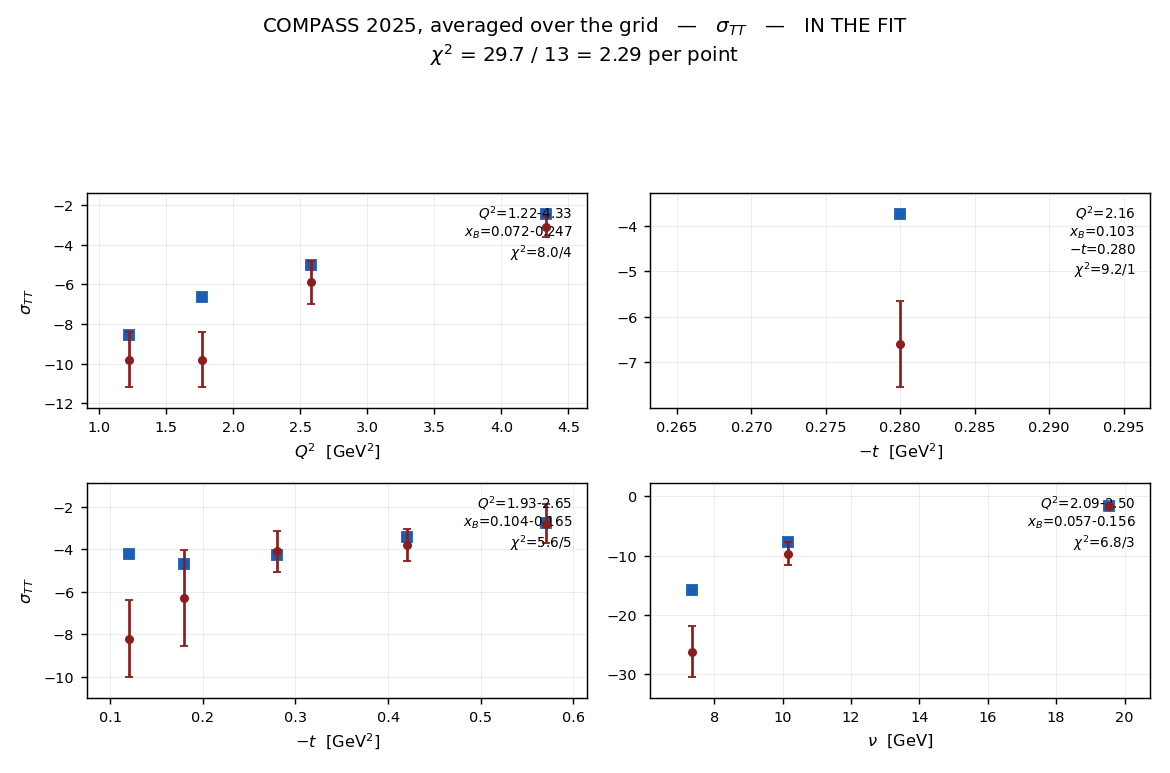
\includegraphics[width=0.72\textwidth]{09_compass_in_TT.png}
\caption{COMPASS 2025.  The model is averaged over the four-dimensional grid
of the measurement, eq.~(16) of the paper, weighted by cell volume: a cell
rectangular in $(Q^2,\nu)$ is not rectangular in $x_B$, and evaluating at the
quoted mean kinematics overshoots by a factor five to eight.}
\end{figure}

\begin{figure}[p]\centering

\includegraphics[width=\textwidth]{01_bsa_demasi_phi_in_A_phi.png}
\caption{De Masi $A_{LU}(\phi)$: all 60 bins, 12 points in $\phi$ each.  The
model supplies the denominator of eq.~(\ref{eq:phidecomp}) from its own
$\sig{LT}$ and $\sig{TT}$, so no free $\beta,\gamma$ are fitted per bin ---
a three-parameter fit per bin is unstable, the denominator passing near zero
in 13 of the 60.}
\end{figure}

\begin{figure}[p]\centering
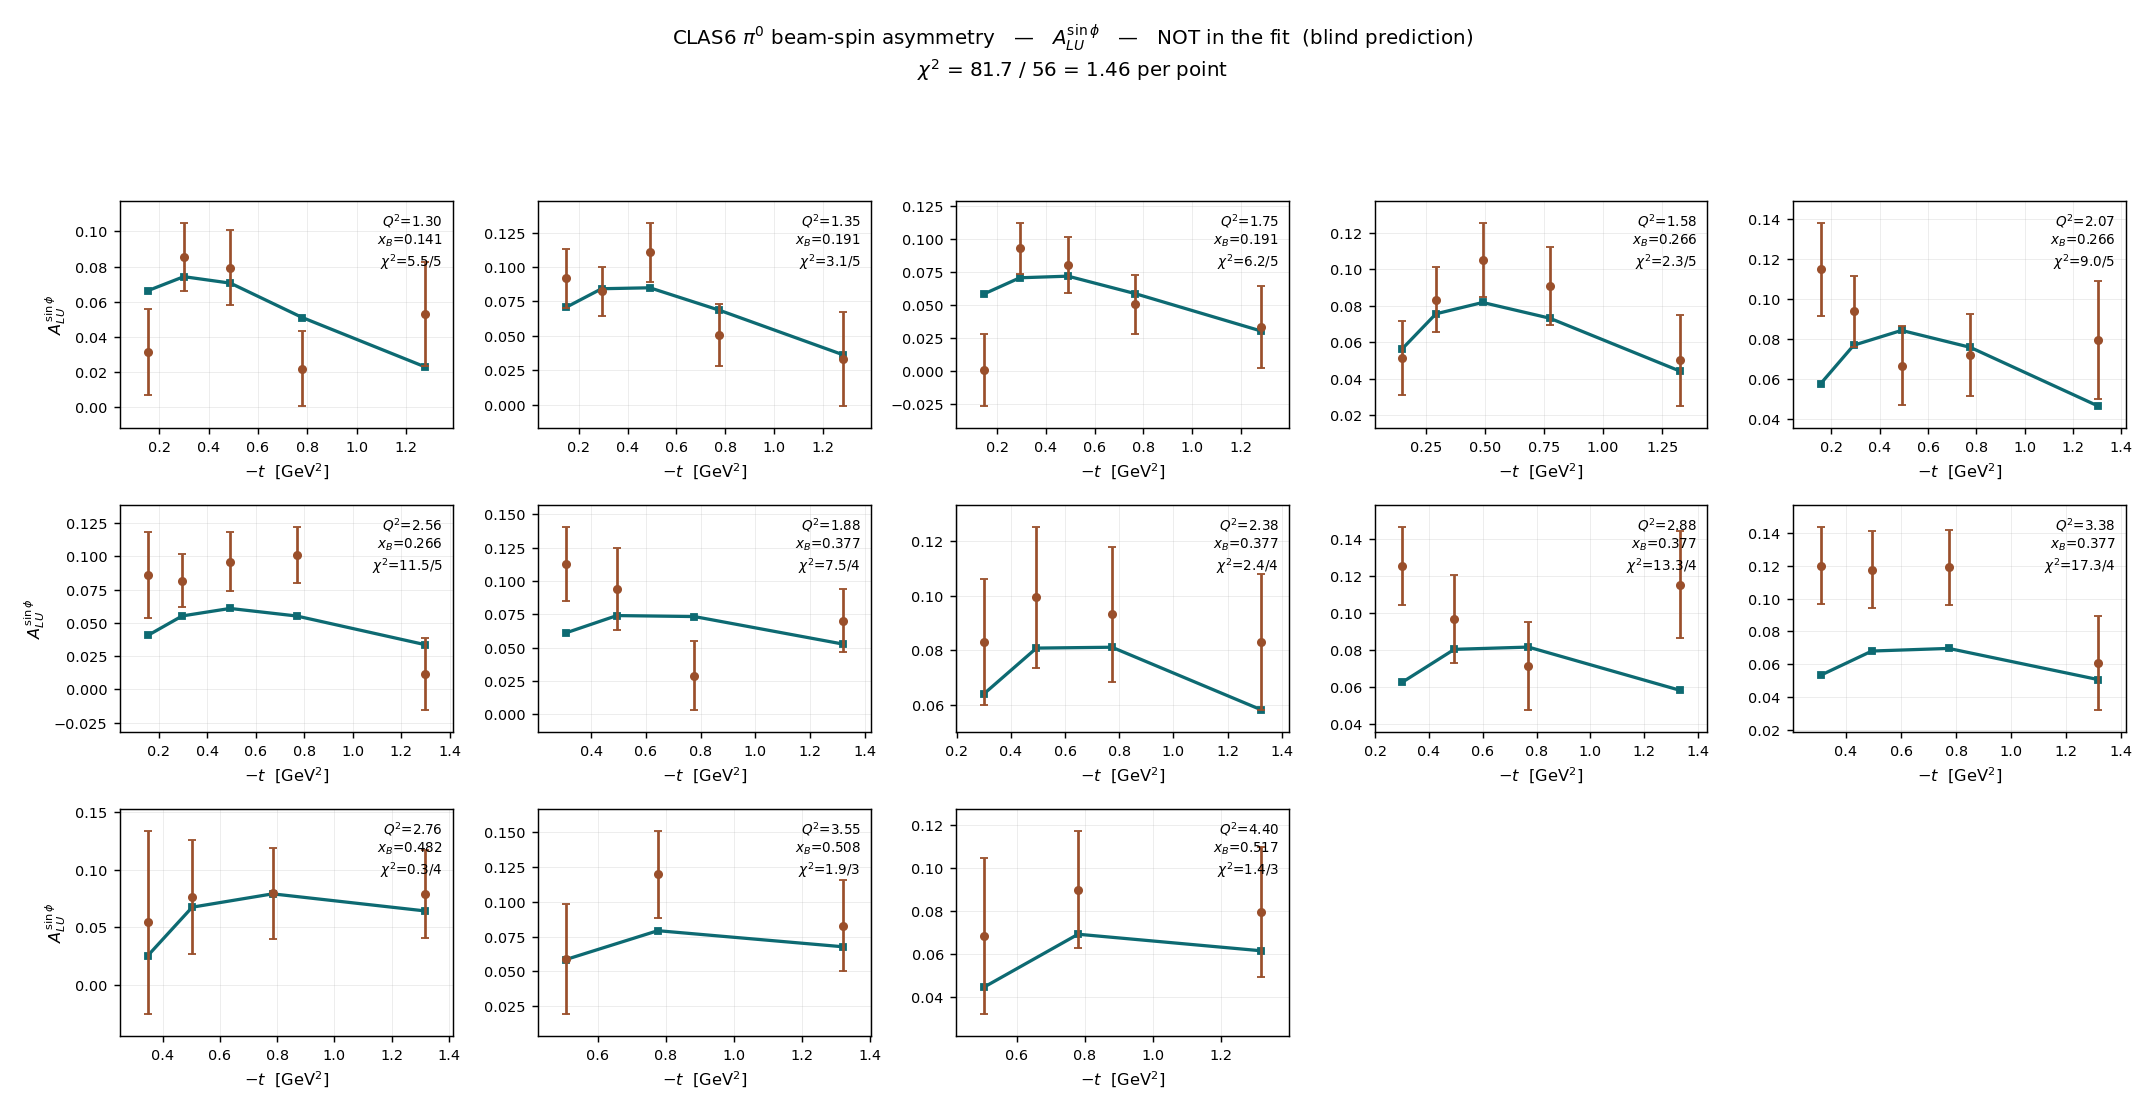
\includegraphics[width=0.75\textwidth]{10_bsa_demasi_out_A_LUsinphi.png}\\
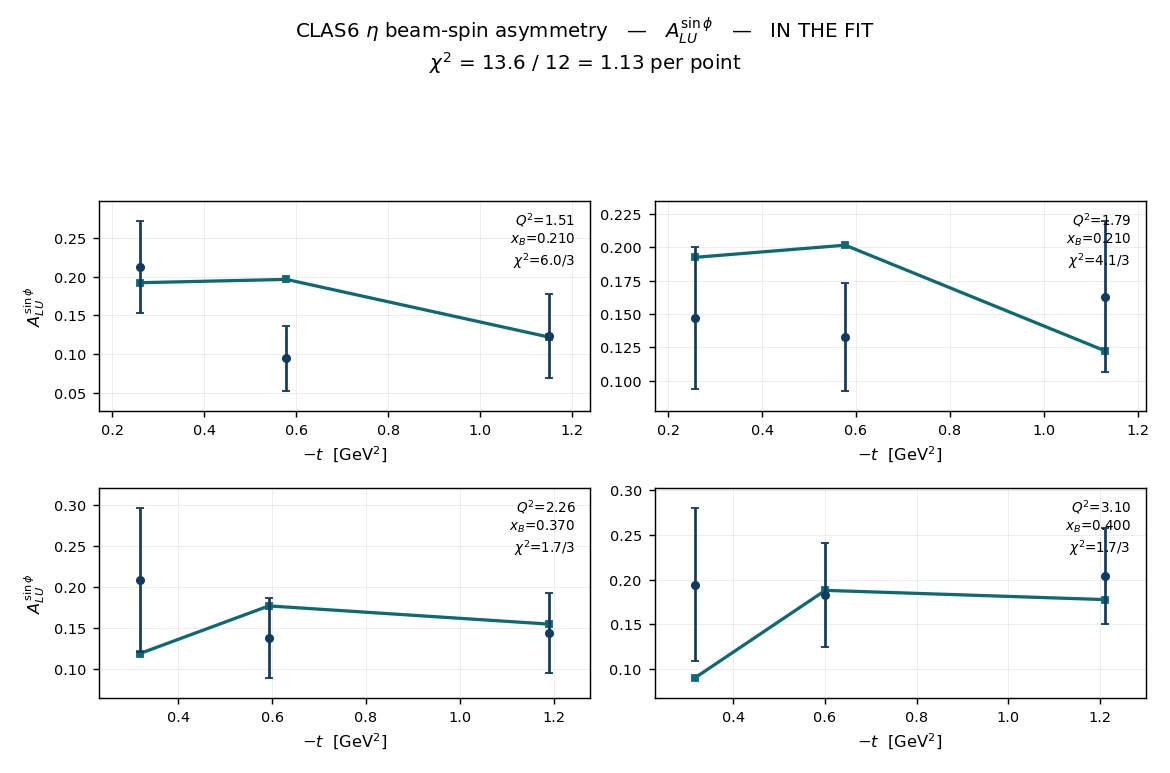
\includegraphics[width=0.75\textwidth]{11_bsa_zhao_in_A_LUsinphi.png}
\caption{Top: the published De Masi $\alpha$, kept out of the fit as the same
measurement as the figure above.  Bottom: the Zhao $\eta$ beam-spin asymmetry,
where the published GK curve is near zero.}
\end{figure}

\begin{figure}[p]\centering

\includegraphics[width=\textwidth]{12_bsa_clas12_in_sigma_LTp_over_sigma_0.png}
\caption{CLAS12 $\sig{LT'}/\sigma_0$.}
\end{figure}

\begin{figure}[p]\centering

\includegraphics[width=0.72\textwidth]{13_eg1_in_ALLc.png}\\

\includegraphics[width=0.72\textwidth]{13_eg1_in_ALLcos.png}
\caption{eg1-dvcs, polarised target: the $A_{LL}$ moments, at the experiment's
two settings.  These are the only observables in the database sensitive to the
relative phase of $T_{01}$ and $U_{01}$; without them it is unconstrained.}
\end{figure}

\begin{figure}[p]\centering

\includegraphics[width=0.72\textwidth]{13_eg1_in_AULsin.png}\\

\includegraphics[width=0.72\textwidth]{13_eg1_in_AULsin2.png}
\caption{eg1-dvcs, the $A_{UL}$ moments.}
\end{figure}

\clearpage
\section*{Reproducing this}

Code, data and the full history are at
\url{https://github.com/vkubarovsky/rc_iter1}.  The fit shown is run
\texttt{\fittag}; its parameter vector is \texttt{runs/\fittag/fitpar.npy} and
every number in the tables above is generated from it by
\texttt{tex/make\_tables.py}, so nothing here is transcribed by hand.  The data
are \texttt{pi0\_eta\_database.xlsx}, md5
\texttt{04c3adf9d6e6b8d2b1b3729f4ff79d1d}; \texttt{export\_db.py --check}
verifies that the CSV cache the fit reads still matches the workbook.

\end{document}
